\documentclass[aspectratio=169]{beamer}

% Use the Conesa Group theme
\usetheme{ConesaGroup}

% Package for better font rendering
\usepackage{lmodern}
\usepackage{microtype}

% Package for graphics
\usepackage{graphicx}

% Package for tables with colors
\usepackage{colortbl}

% Package for mathematics
\usepackage{amsmath}
\usepackage{amssymb}

% Package for bibliography and citations
\usepackage[natbib=true,backend=biber,style=numeric,sorting=none,autocite=superscript]{biblatex}
\addbibresource{references.bib}

% Title information
\title{Profiling the Epigenome Using Long-Read Sequencing}
\subtitle{Journal Club Presentation}
\author[Presenter]{Liu T, Conesa A. Nature Genetics. 2025;57:27-41}
\date{\today}

% Institute information
\institute[]{%
  \begin{flushleft}
    Journal Club Discussion\\
    \small\today
  \end{flushleft}%
}

\begin{document}

% Title page
\begin{frame}[plain]
  \titlepage
\end{frame}

% Table of contents
\begin{frame}{Outline}
  \tableofcontents[hideallsubsections]
\end{frame}

% Section: Overview
\section{Overview}

\begin{frame}{Review Scope and Objectives}
  \begin{block}{What This Review Covers}
    \begin{itemize}
      \item Long-read sequencing (LRS) technologies for epigenomics research
      \item Experimental and computational strategies for characterizing chromatin states
      \item Advantages of LRS over short-read sequencing (SRS) methods
      \item Integration of epigenomic and transcriptomic data for multi-omics studies
    \end{itemize}
  \end{block}

  \vspace{0.3cm}

  \begin{alertblock}{Key Technologies}
    Oxford Nanopore Technologies (ONT) and Pacific Biosciences (PacBio)
  \end{alertblock}
\end{frame}

% Section: Background
\section{Background}

\begin{frame}{Long-Read Sequencing: Key Advantages}
  \begin{columns}[T]
    \begin{column}{0.48\textwidth}
      \begin{block}{Technical Advantages}
        \begin{itemize}
          \item Direct DNA methylation detection
          \item Single-molecule resolution
          \item No PCR amplification needed
          \item Long reads ($>$10 kb)
        \end{itemize}
      \end{block}
    \end{column}
    \begin{column}{0.48\textwidth}
      \begin{block}{Research Applications}
        \begin{itemize}
          \item Haplotype-resolved analysis
          \item Highly repetitive regions (HRRs)
          \item Multi-epigenetic events on same molecule
          \item Complex genomic interactions
        \end{itemize}
      \end{block}
    \end{column}
  \end{columns}
\end{frame}

\begin{frame}{Overview of LRS Epigenomic Strategies}
  \begin{figure}
    \centering
    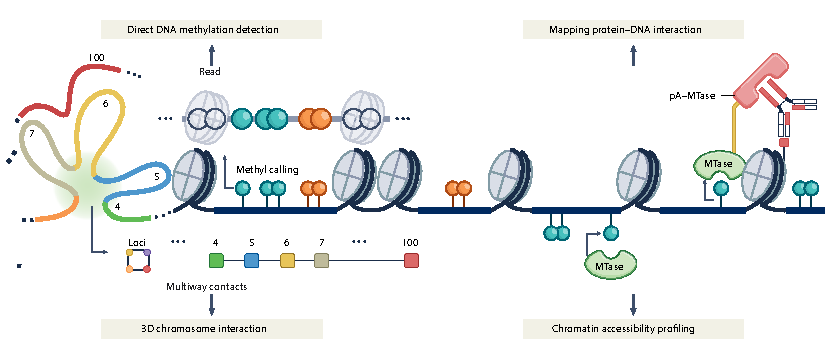
\includegraphics[height=0.5\textheight]{figures/fig1.pdf}

    {\small \textbf{Figure 1} \textbar{} Single-molecule LRS strategies for epigenomic profiling and chromatin interactions.}
  \end{figure}
\end{frame}

\begin{frame}{Four Main LRS Strategies}
  \begin{enumerate}
    \item \textbf{Direct DNA methylation detection}: Sequencing native DNA molecules without bisulfite conversion to detect 5mC, 6mA, and other modifications

    \item \textbf{3D chromosome interaction}: Coupling ligation of long-range interacting regions with LRS to resolve complex 3D topologies and multiway contacts

    \item \textbf{Chromatin accessibility profiling}: Treatment with methyltransferases that mark open regions, followed by LRS to analyze accessibility and nucleosome positioning

    \item \textbf{Protein-DNA interaction mapping}: Fusion of methyltransferases to antibodies for targeted modifications at specific chromatin sites to reveal histone marks and transcription factor binding
  \end{enumerate}
\end{frame}

% Section: DNA Methylation
\section{DNA Methylation Detection}

\begin{frame}{Traditional SRS Methods for DNA Methylation}
  \begin{figure}
    \centering
    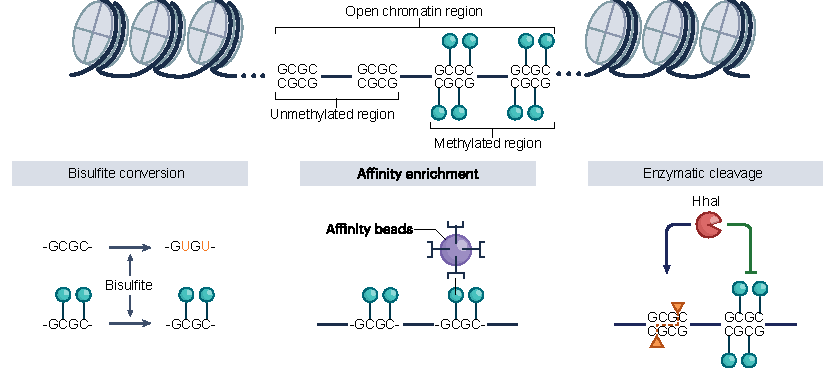
\includegraphics[height=0.5\textheight]{figures/fig2a.pdf}

    {\small \textbf{Figure 2a} \textbar{} SRS methods: bisulfite conversion, affinity enrichment, and enzymatic cleavage.}
  \end{figure}
\end{frame}

\begin{frame}{Limitations of Short-Read Methylation Methods}
  \begin{alertblock}{Key Limitations}
    \begin{itemize}
      \item DNA degradation from bisulfite conversion
      \item Bias toward CpG-rich regions (affinity enrichment)
      \item Limited methylome coverage (restriction enzyme methods)
      \item Cannot distinguish modification types (5mC vs 5hmC vs 6mA)
      \item Poor performance in extreme GC content regions
      \item Difficulty mapping highly repetitive regions
      \item No allele-specific methylation (ASM) detection
    \end{itemize}
  \end{alertblock}
\end{frame}

\begin{frame}{LRS Direct Methylation Detection Workflow}
  \begin{figure}
    \centering
    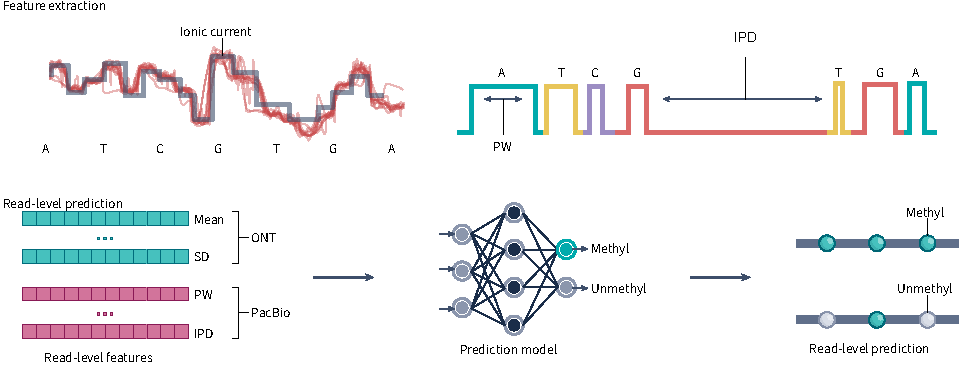
\includegraphics[height=0.5\textheight]{figures/fig2b.pdf}

    {\small \textbf{Figure 2b} \textbar{} LRS methylation detection: feature extraction, read-level prediction, and site-level calling.}
  \end{figure}
\end{frame}

\begin{frame}{Three-Step Methylation Calling Process}
  \begin{enumerate}
    \item \textbf{Feature extraction}
    \begin{itemize}
      \item ONT: Electrical current signals through nanopore
      \item PacBio: Interpulse distance and pulse width
    \end{itemize}

    \item \textbf{Read-level prediction}
    \begin{itemize}
      \item Statistical tests or deep learning models
      \item Tools: Nanopolish, Dorado/Remora, Fibertools, Primrose
    \end{itemize}

    \item \textbf{Site-level prediction}
    \begin{itemize}
      \item Direct count or model-based approach
    \end{itemize}
  \end{enumerate}
\end{frame}

\begin{frame}{Key Methylation Calling Tools}
  \begin{table}
    \small
    \begin{tabular}{|l|l|l|}
      \hline
      \rowcolor{conesaLightGray}
      \textbf{Platform} & \textbf{Tool} & \textbf{Modification Types} \\
      \hline
      ONT & Nanopolish & 5mC \\
      \hline
      ONT & Dorado + Remora & 5mC, 5hmC, 6mA, 4mC (combinations) \\
      \hline
      PacBio & Fibertools & 6mA \\
      \hline
      PacBio & Primrose & 5mC \\
      \hline
    \end{tabular}
  \end{table}

  \vspace{0.3cm}

  \begin{block}{Performance}
    Recent comparisons show both ONT and PacBio offer high-quality CpG methylation detection, with strong correlation to bisulfite sequencing
  \end{block}
\end{frame}

% Section: Chromatin Accessibility
\section{Chromatin Accessibility}

\begin{frame}{Traditional vs LRS Chromatin Accessibility Methods}
  \begin{figure}
    \centering
    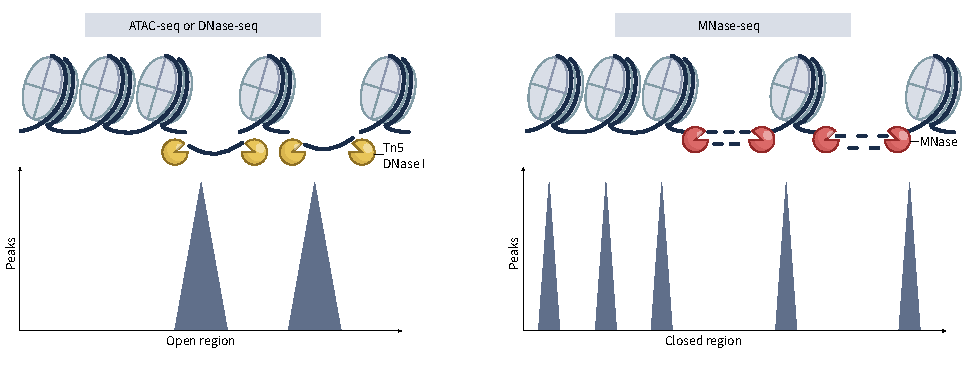
\includegraphics[height=0.5\textheight]{figures/fig3a.pdf}

    {\small \textbf{Figure 3a} \textbar{} Cleavage-based methods: ATAC-seq, DNase-seq, and MNase-seq.}
  \end{figure}
\end{frame}

\begin{frame}{Short-Read Chromatin Accessibility Limitations}
  \begin{block}{Cleavage-Based Methods (ATAC-seq, DNase-seq, MNase-seq)}
    \begin{itemize}
      \item No coordination or co-occurrence of distal accessibility events
      \item Poor performance in segmental duplications and HRRs
    \end{itemize}
  \end{block}

  \begin{block}{Methyltransferase-Based Methods (NOMe-seq)}
    \begin{itemize}
      \item Require bisulfite treatment with lower resolution
      \item Cannot distinguish endogenous from exogenous methylation
    \end{itemize}
  \end{block}
\end{frame}

\begin{frame}{LRS Methyltransferase-Based Accessibility Assays}
  \begin{figure}
    \centering
    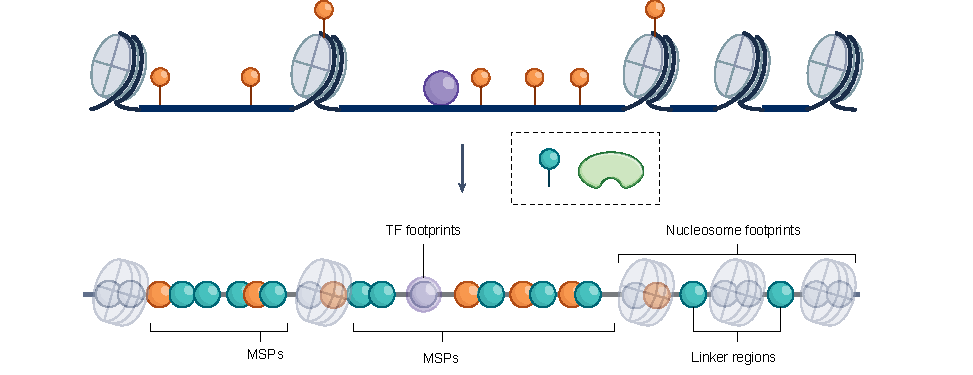
\includegraphics[height=0.5\textheight]{figures/fig3b.pdf}

    {\small \textbf{Figure 3b} \textbar{} DNA methyltransferase treatment followed by direct LRS methylation detection.}
  \end{figure}
\end{frame}

\begin{frame}{LRS Chromatin Accessibility Protocols}
  \begin{table}
    \footnotesize
    \begin{tabular}{|l|l|l|l|}
      \hline
      \rowcolor{conesaLightGray}
      \textbf{Method} & \textbf{Enzyme} & \textbf{Platform} & \textbf{Year} \\
      \hline
      Fiber-seq & Hia5 (6mA) & PacBio, ONT & 2020 \\
      \hline
      SAMOSA & EcoGII (6mA) + MNase & PacBio & 2020 \\
      \hline
      nanoNOMe & CviPI (GpC) & ONT & 2020 \\
      \hline
      SMAC-seq & CviPI + SssI + EcoGII & ONT & 2020 \\
      \hline
      STAM-seq & EcoGII (6mA) & ONT & 2023 \\
      \hline
      SAM-seq & EcoGII (6mA) & ONT & 2024 \\
      \hline
    \end{tabular}
  \end{table}

  \vspace{0.2cm}

  \begin{block}{Key Advantage of 6mA-Based Methods}
    Higher resolution (shorter adenine distances) and no endogenous 6mA in most eukaryotes
  \end{block}
\end{frame}

\begin{frame}{Single-Molecule Chromatin Accessibility Analysis}
  \begin{figure}
    \centering
    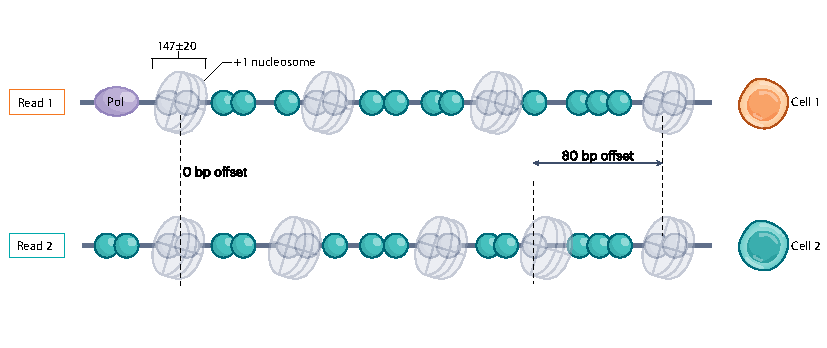
\includegraphics[height=0.5\textheight]{figures/fig4a.pdf}

    {\small \textbf{Figure 4} \textbar{} Data analysis workflow for LRS chromatin accessibility profiling.}
  \end{figure}
\end{frame}

\begin{frame}{Analytical Workflow for Accessibility Data}
  \begin{enumerate}
    \item \textbf{Nucleosome footprints}: Detect ~147 bp inaccessible regions

    \item \textbf{Methylase-sensitive patches (MSPs)}: Identify accessible regions between nucleosomes

    \item \textbf{Machine learning classification}: FIRE tool distinguishes open chromatin from linker DNA

    \item \textbf{Protein footprints}: FiberHMM identifies RNA Pol/TF occupancy

    \item \textbf{Co-actuation analysis}: How one region's accessibility influences adjacent regions
  \end{enumerate}
\end{frame}

% Section: Protein-DNA Interactions
\section{Protein-DNA Interactions}

\begin{frame}{Traditional SRS Protein-DNA Mapping Methods}
  \begin{figure}
    \centering
    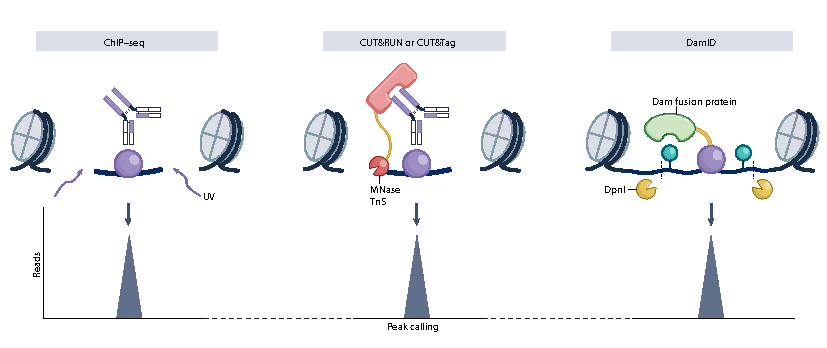
\includegraphics[height=0.5\textheight]{figures/fig5a.pdf}

    {\small \textbf{Figure 5a} \textbar{} SRS methods: ChIP-seq, CUT\&RUN, CUT\&Tag, and DamID.}
  \end{figure}
\end{frame}

\begin{frame}{Limitations of SRS Protein-DNA Methods}
  \begin{alertblock}{Major Limitations}
    \begin{itemize}
      \item Cannot measure multiple protein-binding events on same DNA molecule
      \item No combinatorial binding pattern analysis
      \item Cannot phase haplotype-specific interactions
      \item Poor mapping in highly repetitive regions
      \item DNA methylation information lost during PCR amplification
      \item Limited to pairwise interaction detection
    \end{itemize}
  \end{alertblock}
\end{frame}

\begin{frame}{LRS Antibody-Targeted Methylation Methods}
  \begin{figure}
    \centering
    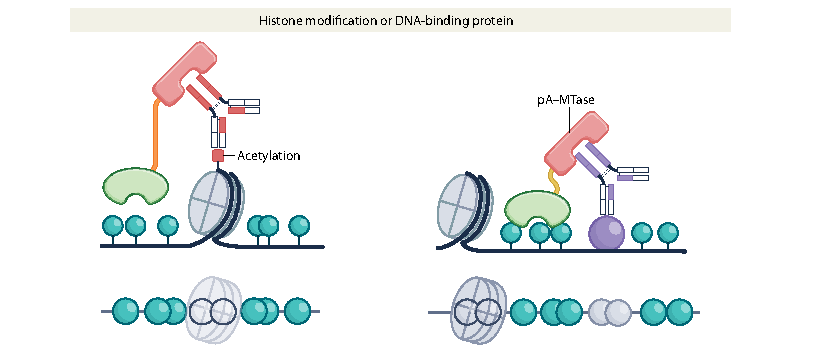
\includegraphics[height=0.5\textheight]{figures/fig5b.pdf}

    {\small \textbf{Figure 5b} \textbar{} LRS protein-DNA interaction mapping: DiMeLo-seq, nanoHiMe-seq, BIND\&MODIFY.}
  \end{figure}
\end{frame}

\begin{frame}{LRS Protein-DNA Interaction Workflow}
  \begin{block}{Protocol Steps}
    \begin{enumerate}
      \item Permeabilize nuclei; add antibody and magnetic beads
      \item Apply pA-methyltransferase fusion protein
      \item Activate with SAM; methylate adenines near target sites
      \item Extract DNA and sequence with ONT/PacBio
      \item Detect methylation as binding markers
    \end{enumerate}
  \end{block}

  \begin{block}{Signal Characteristics}
    Methylation signal decays exponentially (~170 bp half-life)
  \end{block}
\end{frame}

\begin{frame}{Quantitative Advantages: DiMeLo-seq Example}
  \begin{block}{CENP-A Density in Centromeres}
    \begin{itemize}
      \item $>$20-fold coverage in repetitive regions
      \item ~26\% $\pm$ 5\% nucleosomes contain CENP-A
      \item ChIP-seq estimate: ~4\% (1 in 25)
    \end{itemize}
  \end{block}

  \vspace{0.3cm}

  \begin{alertblock}{Key Advantage}
    Absolute frequency measurements without PCR bias
  \end{alertblock}
\end{frame}

\begin{frame}{Single-Molecule Histone Modification Analysis}
  \begin{block}{BIND\&MODIFY Approach}
    Categorize into heavy ($>$75\%), medium (25--75\%), light ($<$25\%) states
  \end{block}

  \begin{block}{Key Findings}
    \begin{itemize}
      \item Heavy/medium H3K27me3 = lower expression
      \item H3K27me3 + CpG methylation on same fibers
    \end{itemize}
  \end{block}
\end{frame}

% Section: 3D Genome
\section{3D Genome Organization}

\begin{frame}{Long-Read 3D Genome Methods}
  \begin{block}{LRS-Based 3D Methods}
    \begin{table}
      \small
      \begin{tabular}{|l|l|l|}
        \hline
        \rowcolor{conesaLightGray}
        \textbf{Method} & \textbf{Platform} & \textbf{Capability} \\
        \hline
        C-walk & PacBio & First LRS 3D genome \\
        \hline
        MC-4C & PacBio, ONT & Targeted loci \\
        \hline
        MC-3C & PacBio & All-vs-all \\
        \hline
        Pore-C & ONT & Multiway contacts \\
        \hline
        HiPore-C & ONT & Enhanced resolution \\
        \hline
      \end{tabular}
    \end{table}
  \end{block}

  \begin{alertblock}{Major Advantage}
    Multiway chromatin interactions in single molecules
  \end{alertblock}
\end{frame}

\begin{frame}{Pore-C Multiway Interaction Analysis}
  \begin{block}{Integration Potential}
    \textbf{Transcription clusters}: Colocalized loci coordinating expression
  \end{block}

  \begin{block}{Current Limitations}
    \begin{itemize}
      \item Tools not designed for single-molecule
      \item 3D loops are dynamic and short-lived
    \end{itemize}
  \end{block}
\end{frame}

% Section: Multi-omics
\section{Multi-Omics Integration}

\begin{frame}{LRS in Transcriptomics}
  \begin{columns}[T]
    \begin{column}{0.48\textwidth}
      \begin{block}{ONT}
        \begin{itemize}
          \item $>$100M reads/flow cell
          \item Direct RNA-seq (m6A)
          \item Real-time acquisition
        \end{itemize}
      \end{block}
    \end{column}
    \begin{column}{0.48\textwidth}
      \begin{block}{PacBio}
        \begin{itemize}
          \item $>$99\% HiFi accuracy
          \item 100M reads/run
          \item Isoform resolution
        \end{itemize}
      \end{block}
    \end{column}
  \end{columns}

  \vspace{0.3cm}

  \begin{block}{Emerging Applications}
    Nascent-seq, Ribo-STAMP, single-cell and spatial RNA-seq
  \end{block}
\end{frame}

\begin{frame}{Toward Multi-Omics Applications}
  \begin{block}{Examples}
    \begin{itemize}
      \item Hi-C + LRS + RNA-seq
      \item Synchronized genome, methylome, epigenome, transcriptome
      \item scNanoCOOL-seq: Single-cell profiling
    \end{itemize}
  \end{block}

  \begin{alertblock}{Key Challenge}
    Cannot map modalities to same molecules
  \end{alertblock}
\end{frame}

\begin{frame}{Analytical Challenges for Multi-Omics}
  \begin{block}{Experimental Needs}
    Higher signal-to-noise, coverage, reduced costs
  \end{block}

  \begin{block}{Computational Needs}
    \begin{itemize}
      \item Benchmarks and signal extraction
      \item Co-occurrence detection
      \item Integration frameworks
    \end{itemize}
  \end{block}
\end{frame}

% Section: Current State
\section{Current State and Gaps}

\begin{frame}{Current State of Knowledge}
  \begin{block}{LRS Achievements}
    \begin{itemize}
      \item Direct detection of 5mC, 6mA, 4mC, 5hmC
      \item Single-molecule chromatin states
      \item Haplotype-resolved analysis
      \item Mapping repetitive regions
      \item Multiway chromatin interactions
      \item Quantitative protein-DNA without PCR bias
    \end{itemize}
  \end{block}
\end{frame}

\begin{frame}{Gaps and Challenges}
  \begin{alertblock}{Technical}
    \begin{itemize}
      \item High costs, limited coverage
      \item Model retraining with updates
      \item Signal decay, limited standardization
    \end{itemize}
  \end{alertblock}

  \begin{alertblock}{Analytical}
    \begin{itemize}
      \item TF motif degeneracy
      \item Lack of single-molecule 3D tools
      \item Cannot link DNA to RNA
    \end{itemize}
  \end{alertblock}
\end{frame}

% Section: Future Directions
\section{Future Directions}

\begin{frame}{Future Directions}
  \begin{enumerate}
    \item \textbf{Technology}: Universal models, cost reduction, enrichment

    \item \textbf{Analytics}: Integration frameworks, co-occurrence detection, TF assignment

    \item \textbf{Biology}: Link chromatin to transcription, combinatorial regulation, disease
  \end{enumerate}
\end{frame}

% Section: Conclusion
\section{Conclusion}

\begin{frame}{Take-Home Messages}
  \begin{alertblock}{Key Points}
    \begin{enumerate}
      \item Direct detection without conversion/amplification

      \item Single-molecule, haplotype-resolved

      \item Overcomes SRS limitations

      \item Multi-omics profiling

      \item Linking chromatin to transcription
    \end{enumerate}
  \end{alertblock}
\end{frame}

\begin{frame}{Discussion Questions}
  \begin{enumerate}
    \item How might single-molecule data change our understanding of gene regulation?

    \item What computational challenges need addressing?

    \item Which biological questions could benefit from LRS?

    \item How to balance cost vs coverage?

    \item How to link DNA to RNA molecules?
  \end{enumerate}
\end{frame}

\begin{frame}
  \begin{center}
    \large\textbf{Thank you for your attention!}

    \vspace{0.5cm}

    \normalsize
    Questions and Discussion?
  \end{center}
\end{frame}

% References slide
\begin{frame}[allowframebreaks]{References}
  \printbibliography
\end{frame}

\end{document}
